\chapter{User Manuals}

\begin{figure}[h]
\begin{center}
  % Requires \usepackage{graphicx}
  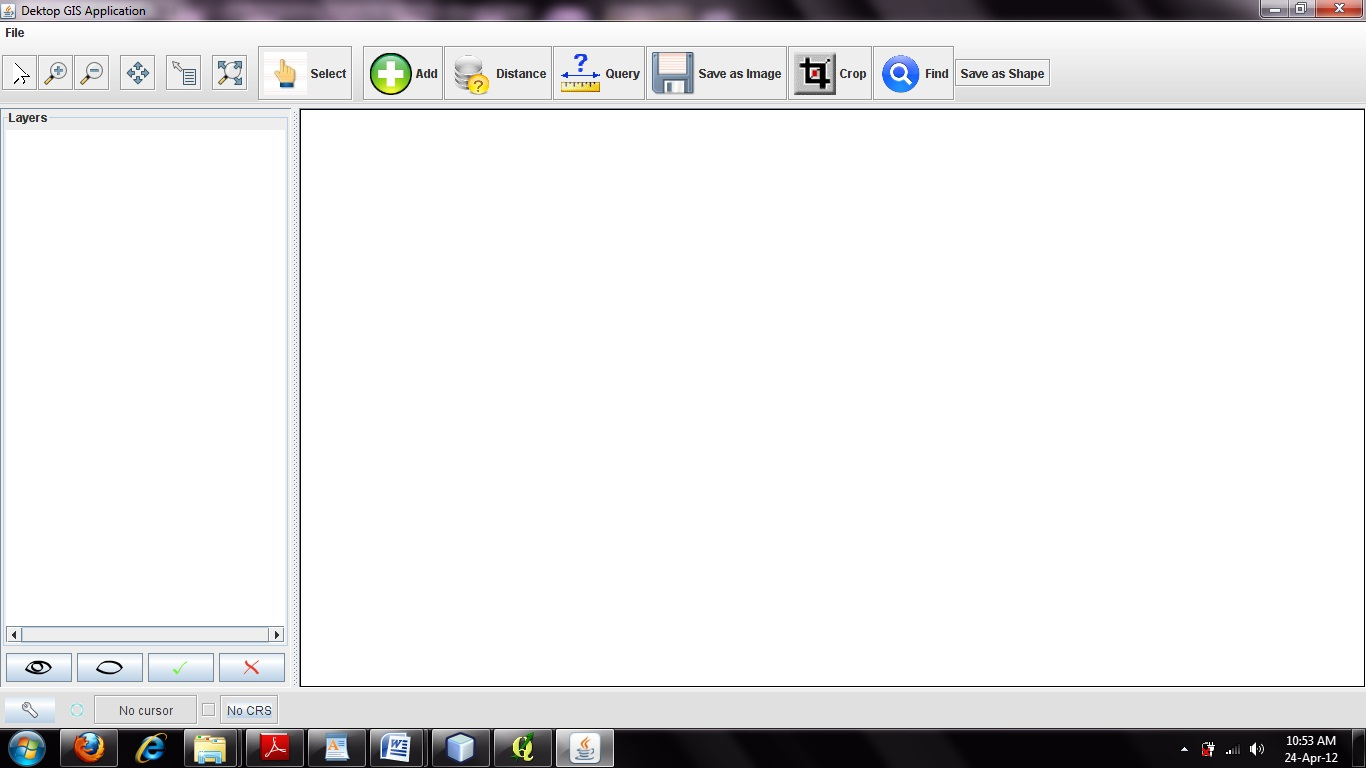
\includegraphics[scale=0.43] {1.jpg}
  \caption[Screenshot - Outlook]{Main outlook of Application}
\end{center}
\end{figure}
Description: Above is the basic outlook of Application.The left side is Layer Table.The main area is MapFrame.On the Top menubar and toolbar for performing various functionality.

\newpage
\begin{figure}[h]
\begin{center}
  % Requires \usepackage{graphicx}
  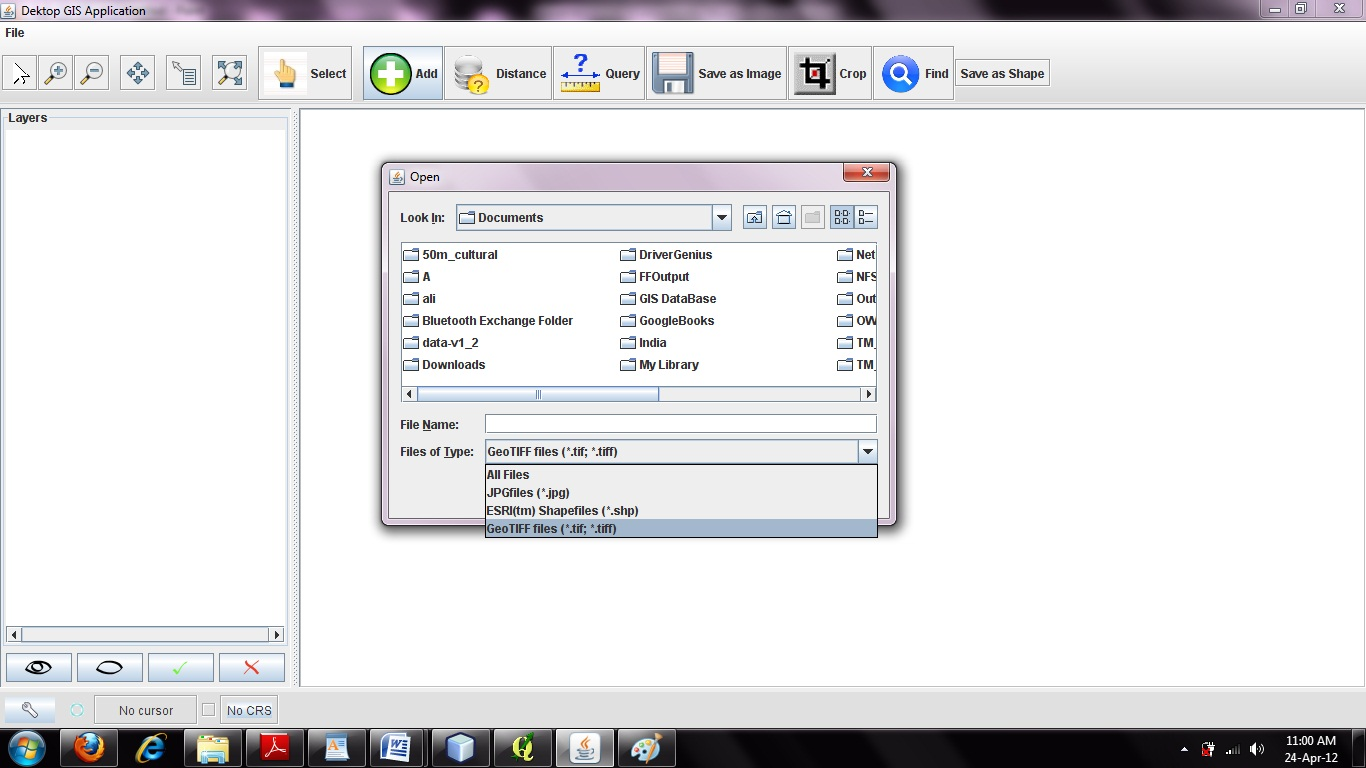
\includegraphics[scale=0.43] {2.jpg}
  \caption[Screenshot - Add Layer]{Add button Function}
\end{center}
\end{figure}
Description: Above is the outcome when user clicked on the “ADD” button. It prompt for selecting the input of Raster(.jpg,.tiff) as well as Vector(.shp) data.

\newpage
\begin{figure}[h]
\begin{center}
  % Requires \usepackage{graphicx}
  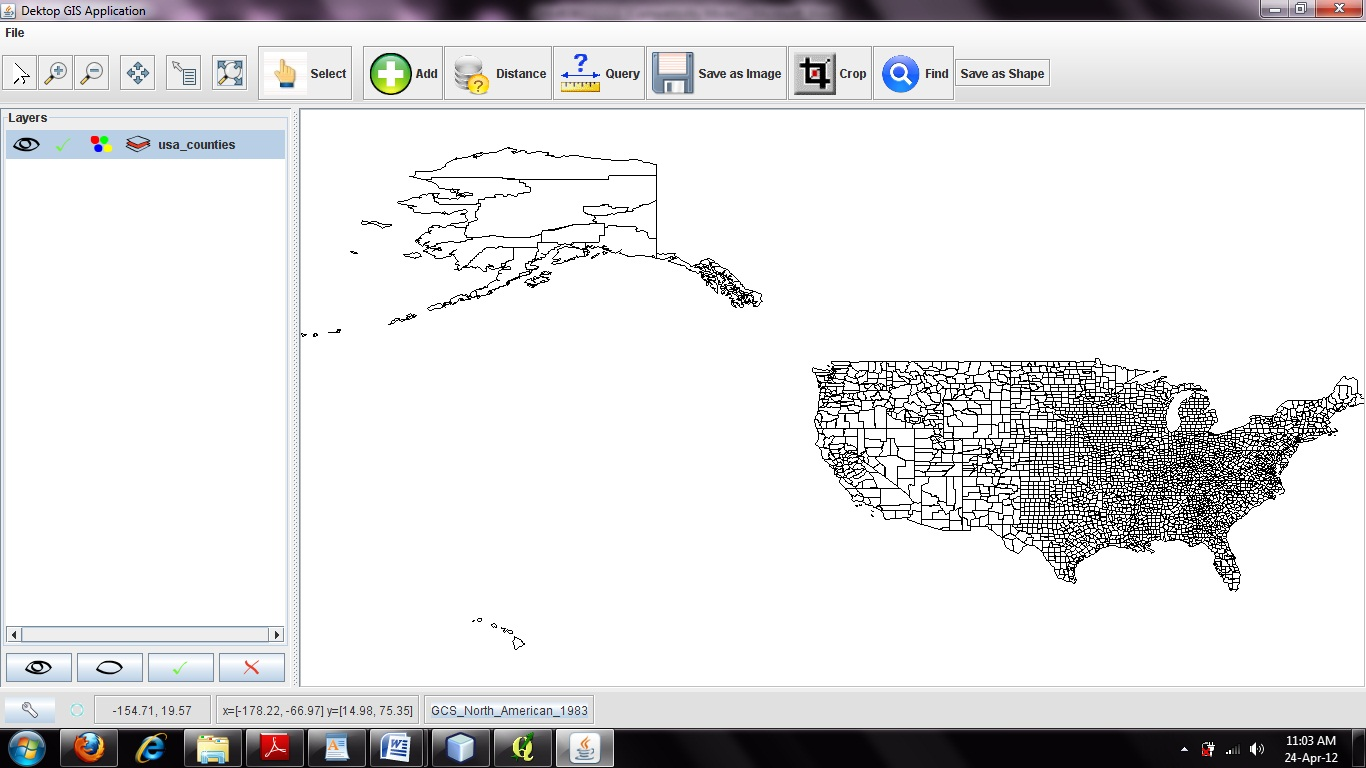
\includegraphics[scale=0.43] {3.jpg}
  \caption[Screenshot - View Shapefile]{Basic rendering of Simple Map}
\end{center}
\end{figure}
Description: Above is the output when user select some shape file from the JFiledatachooser.In the Layer Table he/she can see the option to remove,select/deselect,set layer style and toggling visibility option. At the bottom he/she can see the status bar which shows the CRS of the current Layer rendered in MapFrame.

\newpage


\begin{figure}[h]
\begin{center}
  % Requires \usepackage{graphicx}
  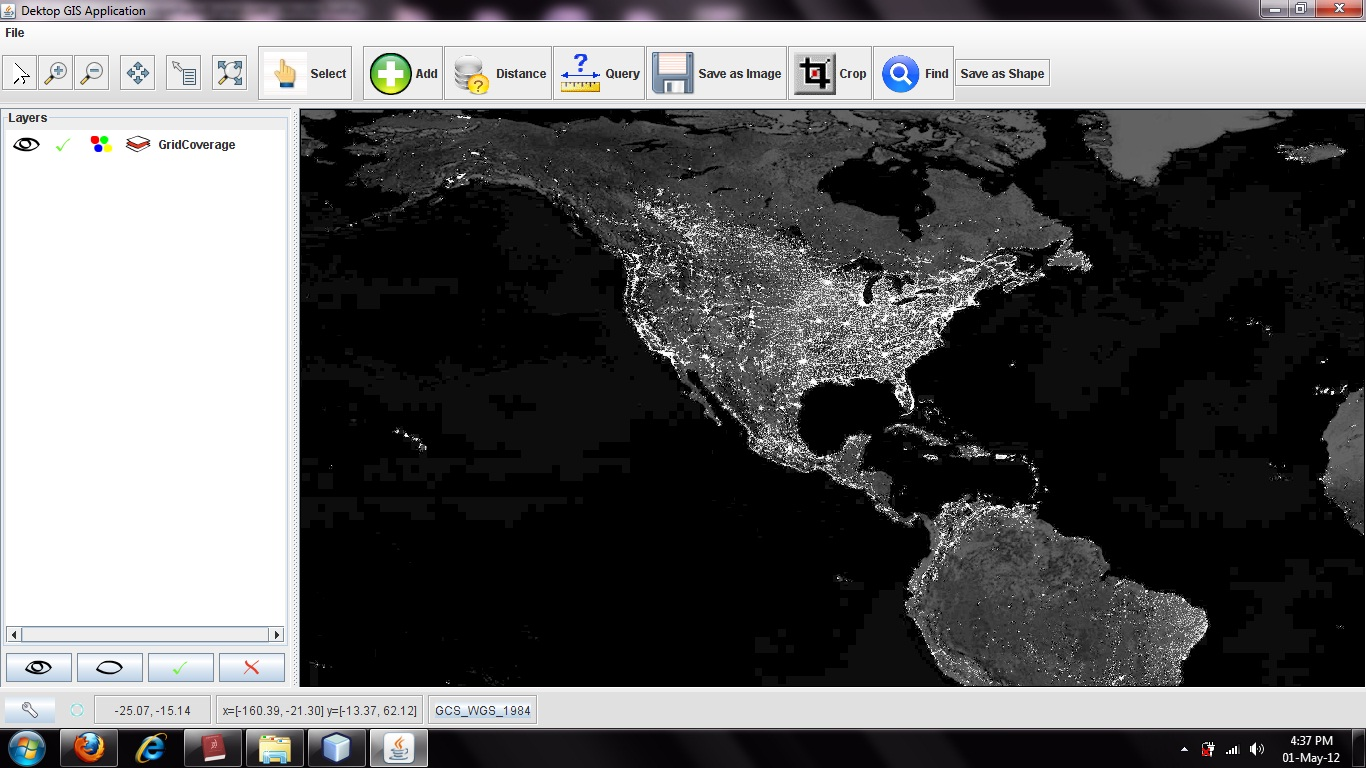
\includegraphics[scale=0.43] {4.jpg}
  \caption[Screenshot - View Image]{Basic rendering of Raster data}
\end{center}
\end{figure}
Description: Above is rendering of geo-referenced JPEG file.

\newpage
\begin{figure}[h]
\begin{center}
  % Requires \usepackage{graphicx}
  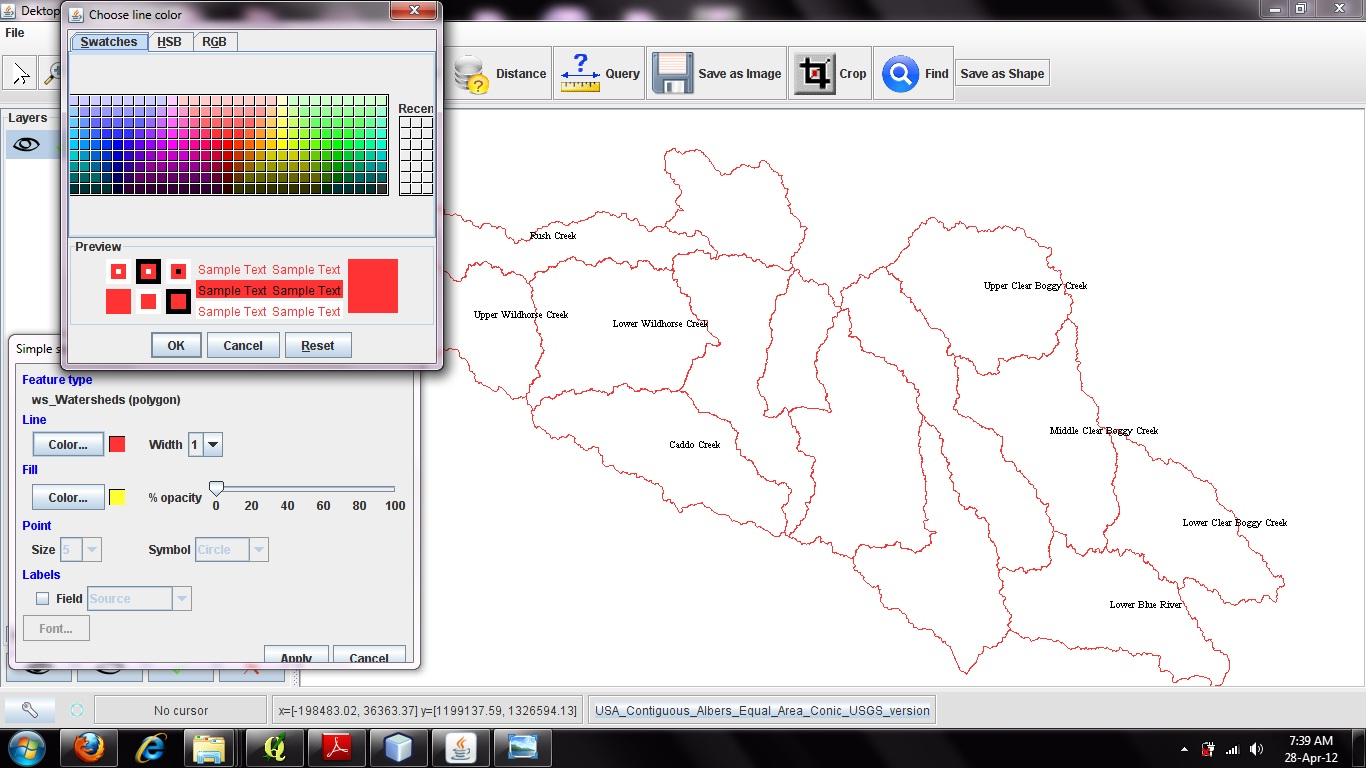
\includegraphics[scale=0.43] {5.jpg}
  \caption[Screenshot - Style]{Use of Layer table option’s function}
\end{center}
\end{figure}
Description: Above is the use of functionality provided by Layer table option. User can color the boundy of Map. User can feel the color in Map also. User can Lable the Map using attribute Table’s field.

\newpage
\begin{figure}[h]
\begin{center}
  % Requires \usepackage{graphicx}
  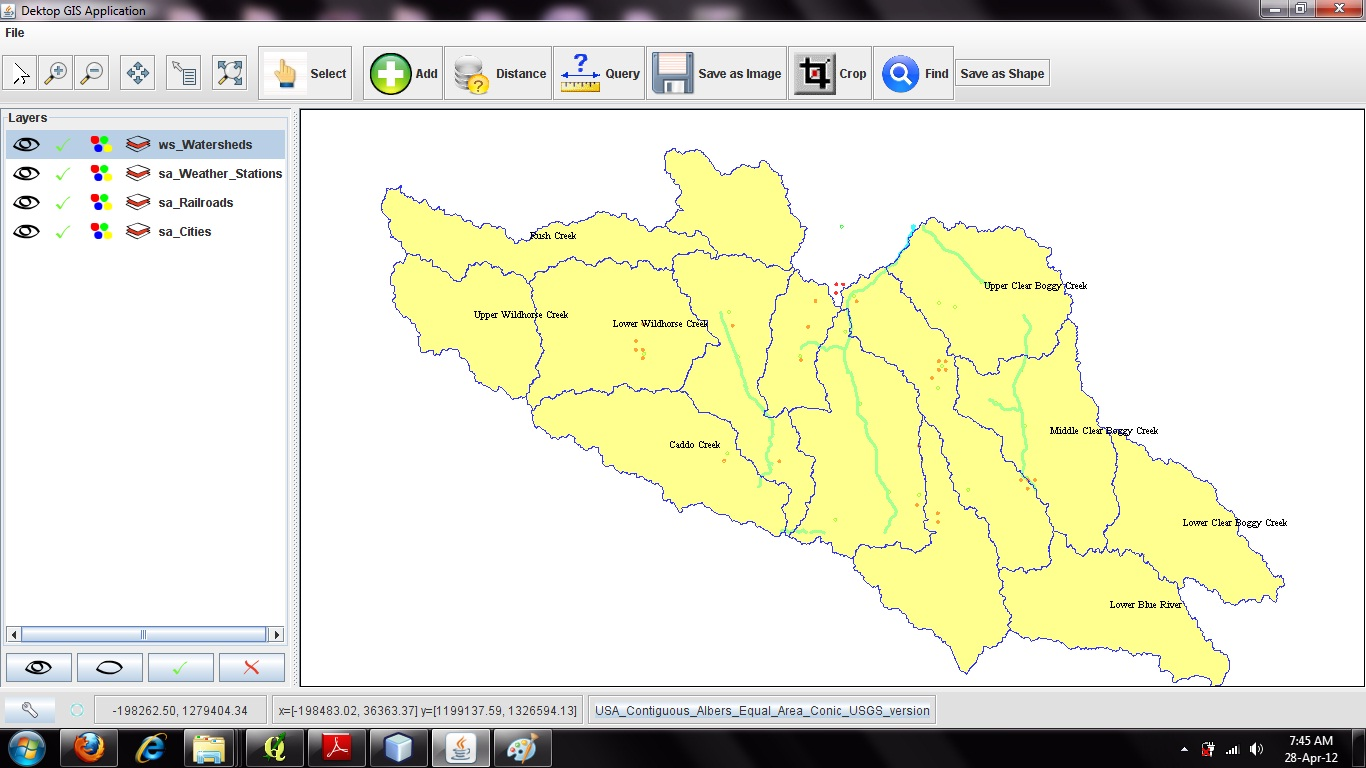
\includegraphics[scale=0.43] {6.jpg}
  \caption[Screenshot - Multilayering]{Multilayering}
\end{center}
\end{figure}
Description: Above is output of multilayering with two vector and one raster layer. User have colored the vector data and labeling it.

\newpage
\begin{figure}[h]
\begin{center}
  % Requires \usepackage{graphicx}
  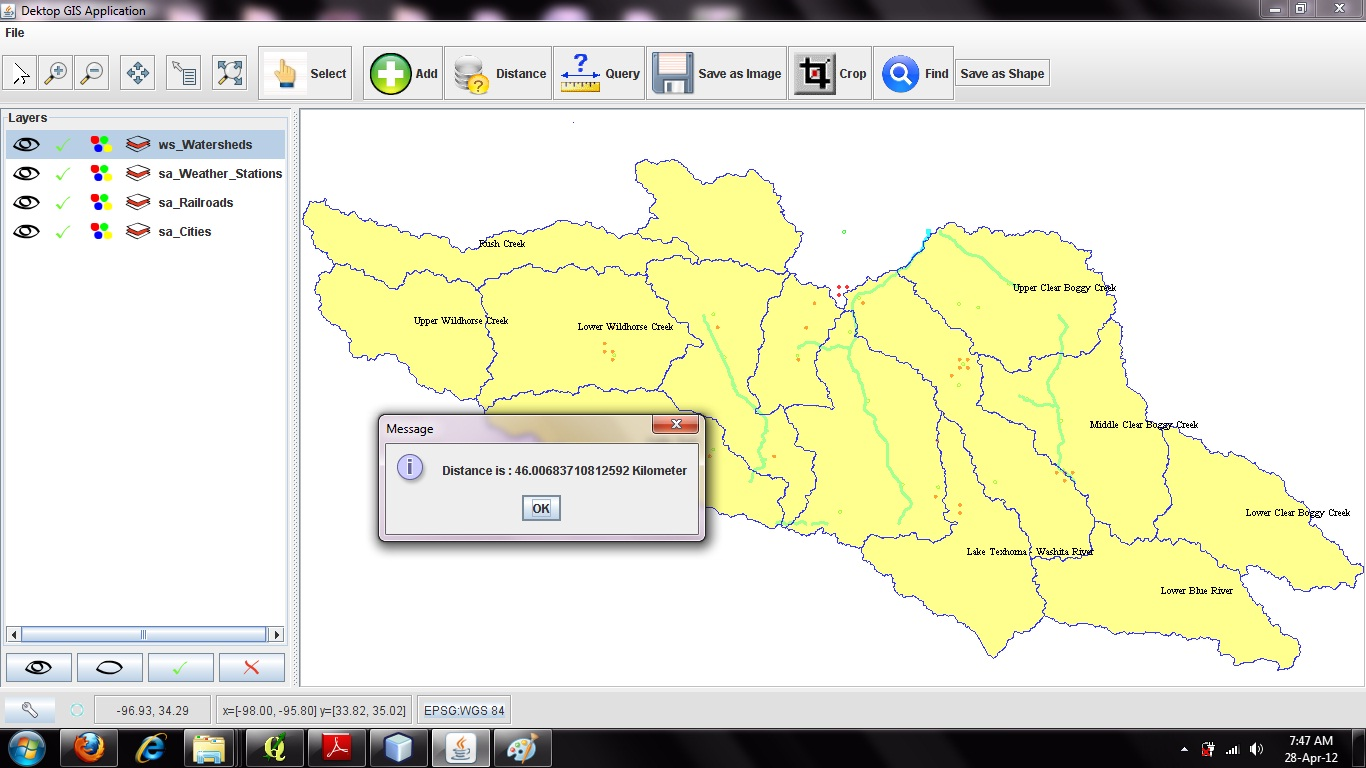
\includegraphics[scale=0.43] {7.jpg}
  \caption[Screenshot - Distance]{Distance feature}
\end{center}
\end{figure}
Description: Above feature is useful to calculate distance between two points in Map in kilometers.

\newpage

\begin{figure}[h]
\begin{center}
  % Requires \usepackage{graphicx}
  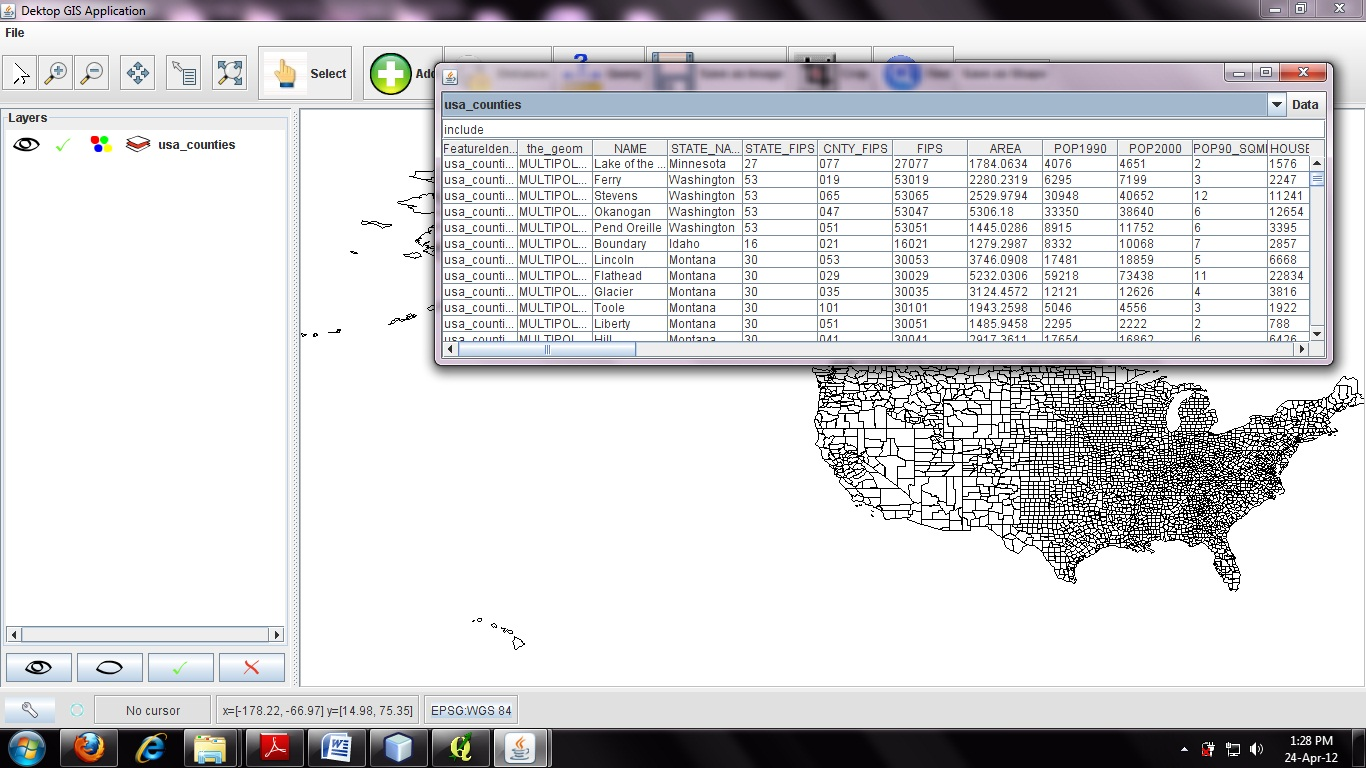
\includegraphics[scale=0.43] {8.jpg}
  \caption[Screenshot - Attribute table]{Attribute Table of  Map}
\end{center}
\end{figure}
Description: Above is the display of attribute table of a given Map in Layer  table.
\newpage
\begin{figure}[h]
\begin{center}
  % Requires \usepackage{graphicx}
  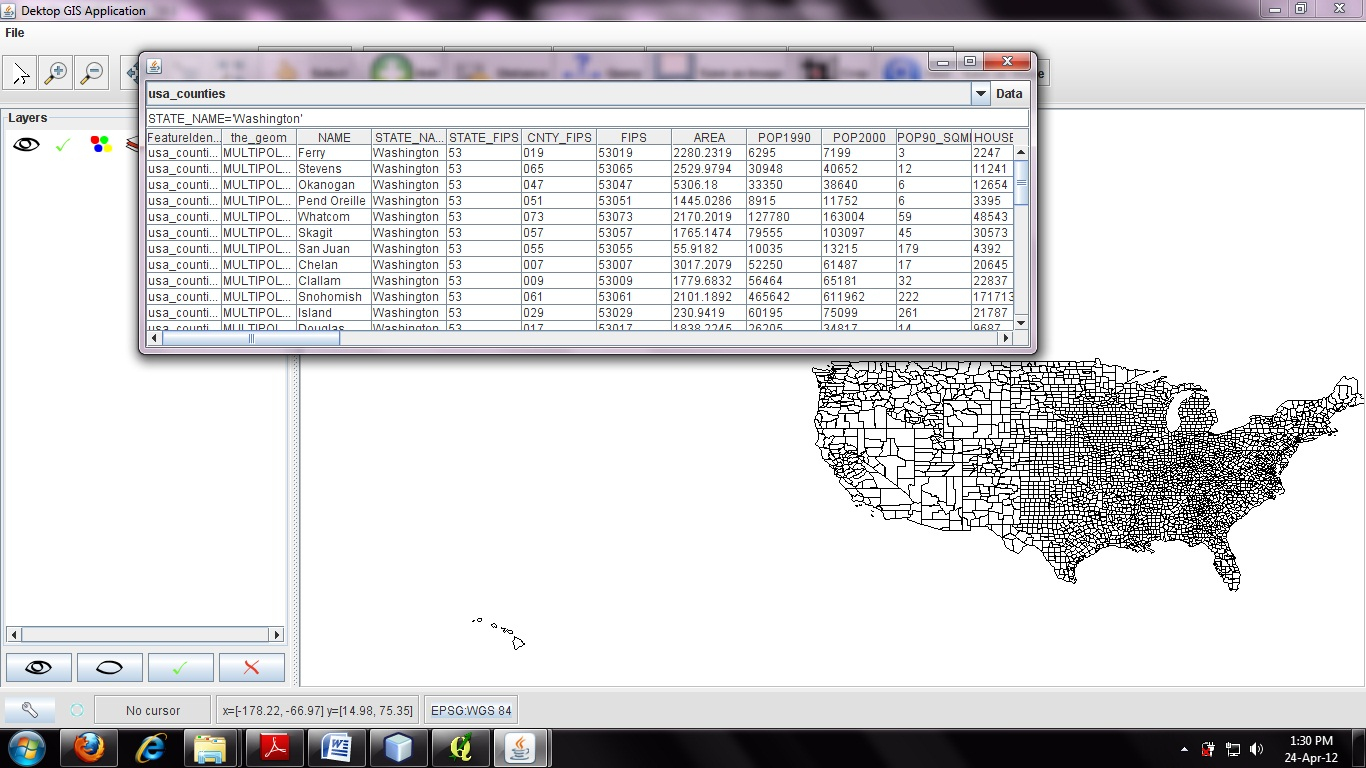
\includegraphics[scale=0.43] {9.jpg}
  \caption[Screenshot - Query]{Query performance on Attribute}
\end{center}
\end{figure}
\newpage
\begin{figure}[h]
\begin{center}
  % Requires \usepackage{graphicx}
  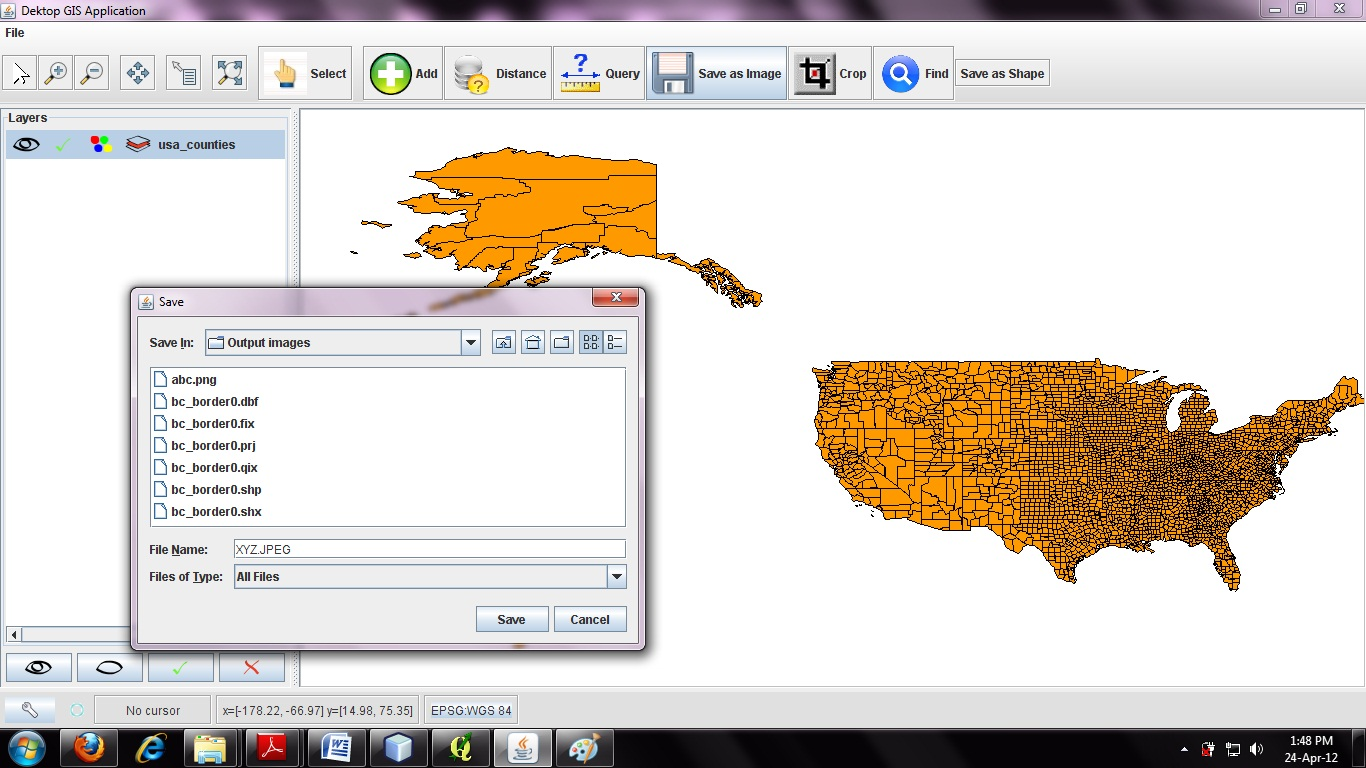
\includegraphics[scale=0.43] {10.jpg}
  \caption[Screenshot - Save]{Save as Image}
\end{center}
\end{figure}
Description: Above it is seen that the user can save the file as Image.(Jpeg,Tiff,Bmp,Png) and Many other format.
\newpage


\begin{figure}[h]
\begin{center}
  % Requires \usepackage{graphicx}
  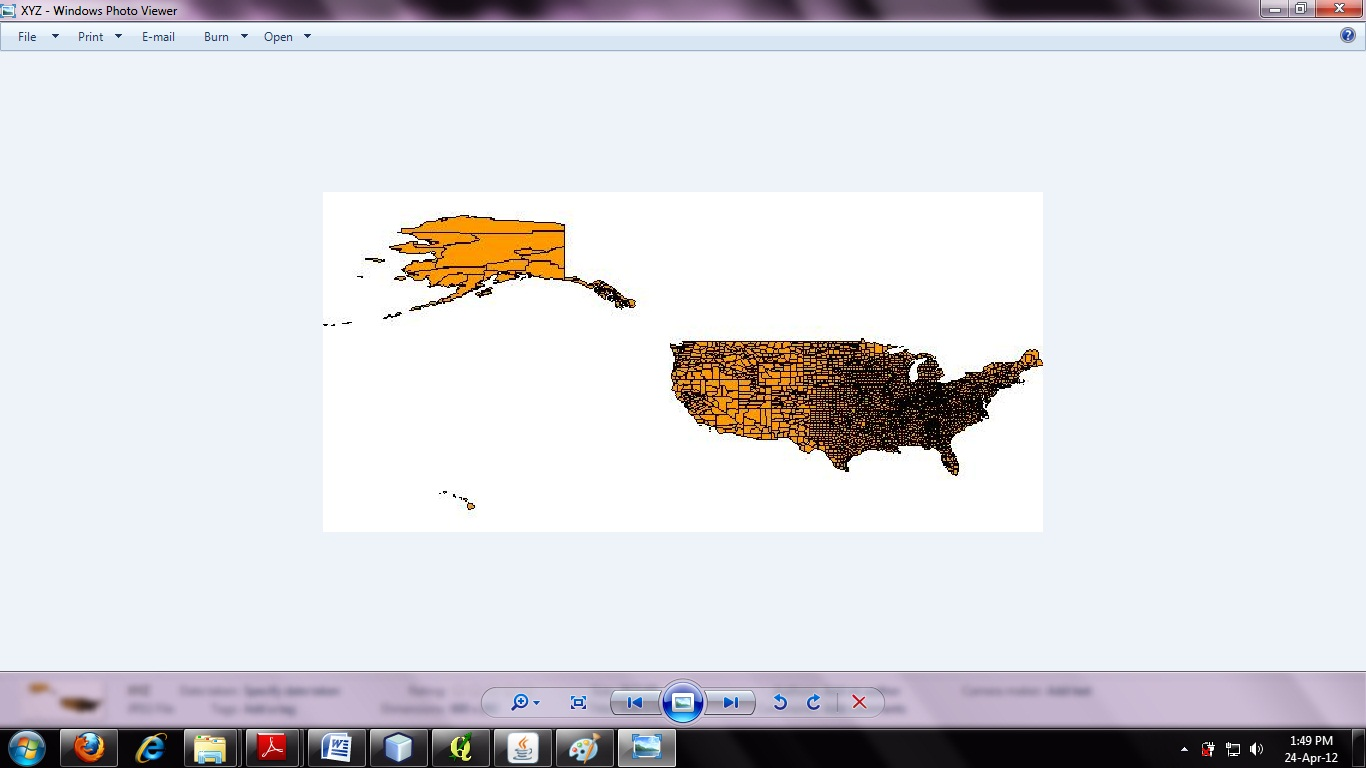
\includegraphics[scale=0.43] {11.jpg}
  \caption[Screenshot - Output Image]{Output as Image}
\end{center}
\end{figure}
Description: Above is output of image file stored in previous case.

\newpage
\begin{figure}[h]
\begin{center}
  % Requires \usepackage{graphicx}
  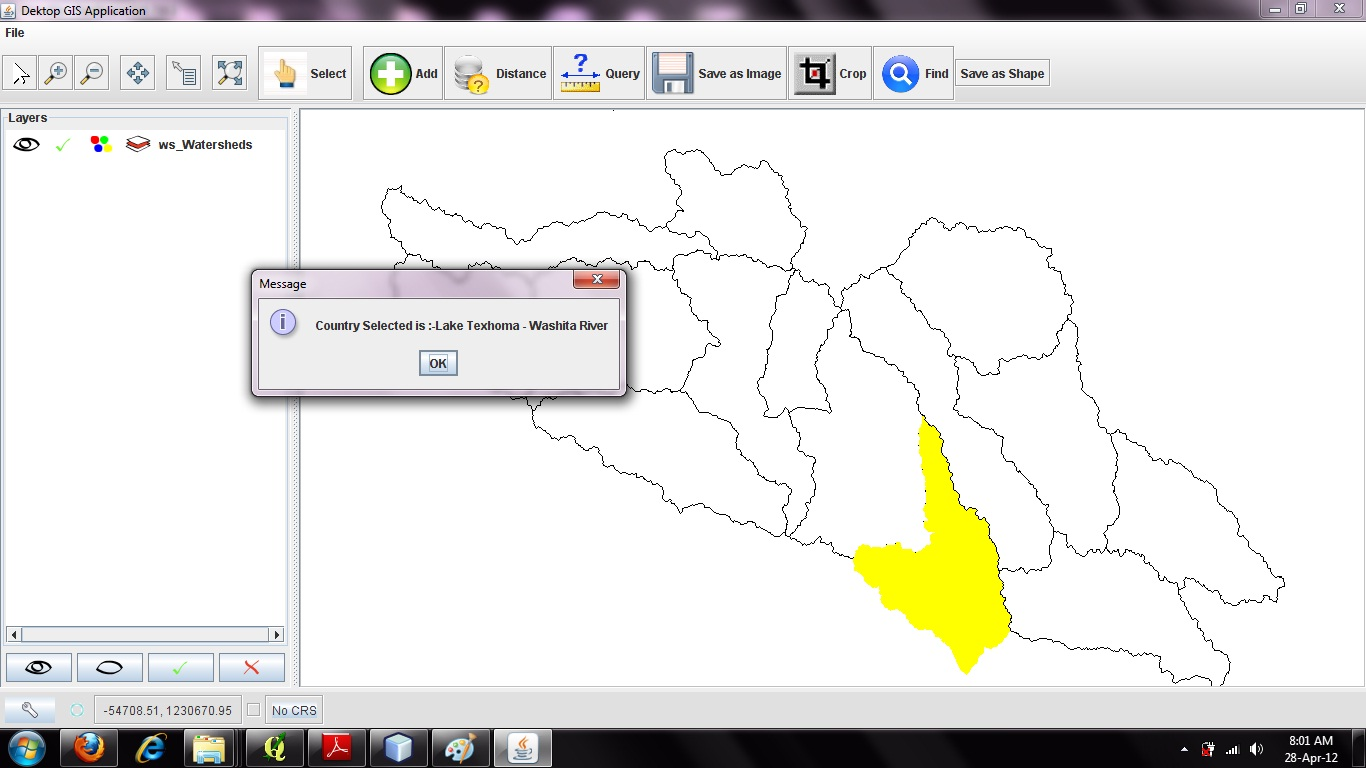
\includegraphics[scale=0.43] {12.jpg}
  \caption[Screenshot - Selection]{Selection feature}
\end{center}
\end{figure}
Description: User can select particular country from map and the name of that selected feature is prompted.
\newpage




\begin{figure}[h]
\begin{center}
  % Requires \usepackage{graphicx}
  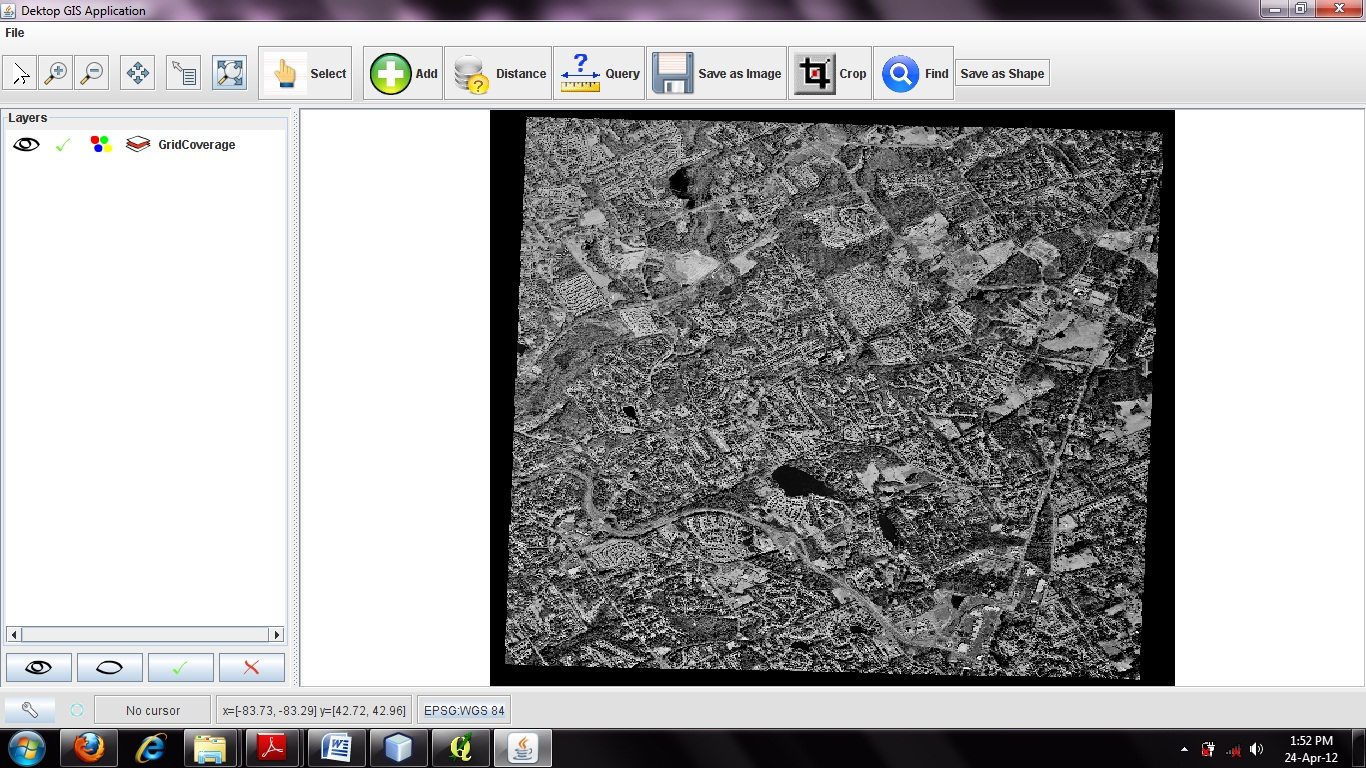
\includegraphics[scale=0.43] {13.jpg}
  \caption[Screenshot - GeoTiff File]{Open GeoTiff file}
\end{center}
\end{figure}
Description: User can open geo referenced TIFF file.

\newpage
\begin{figure}[h]
\begin{center}
  % Requires \usepackage{graphicx}
  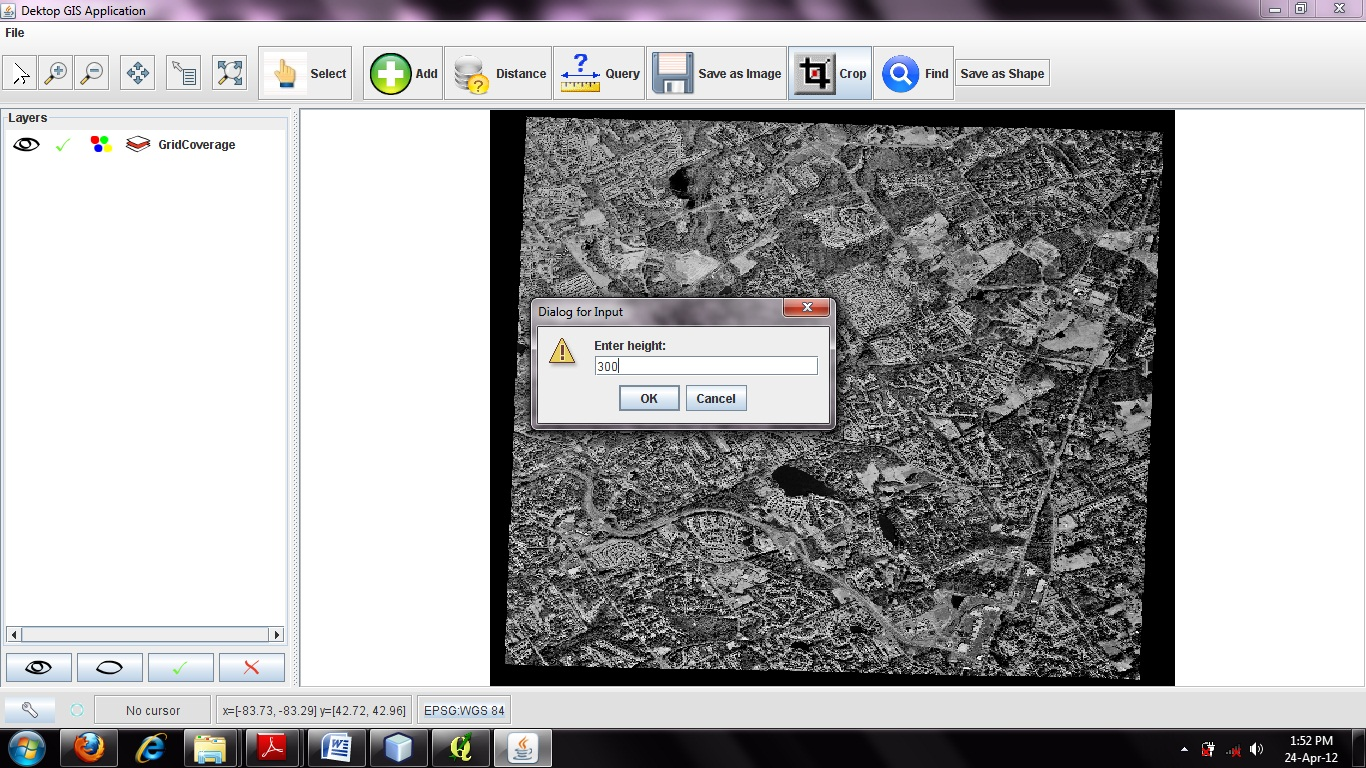
\includegraphics[scale=0.43] {14.jpg}
  \caption[Screenshot - Crop]{Crop the GEOTiff file}
\end{center}
\end{figure}
Description: User have to set parameter for cropping the image like width,height and the point from where to crop.
\newpage

\begin{figure}[h]
\begin{center}
  % Requires \usepackage{graphicx}
  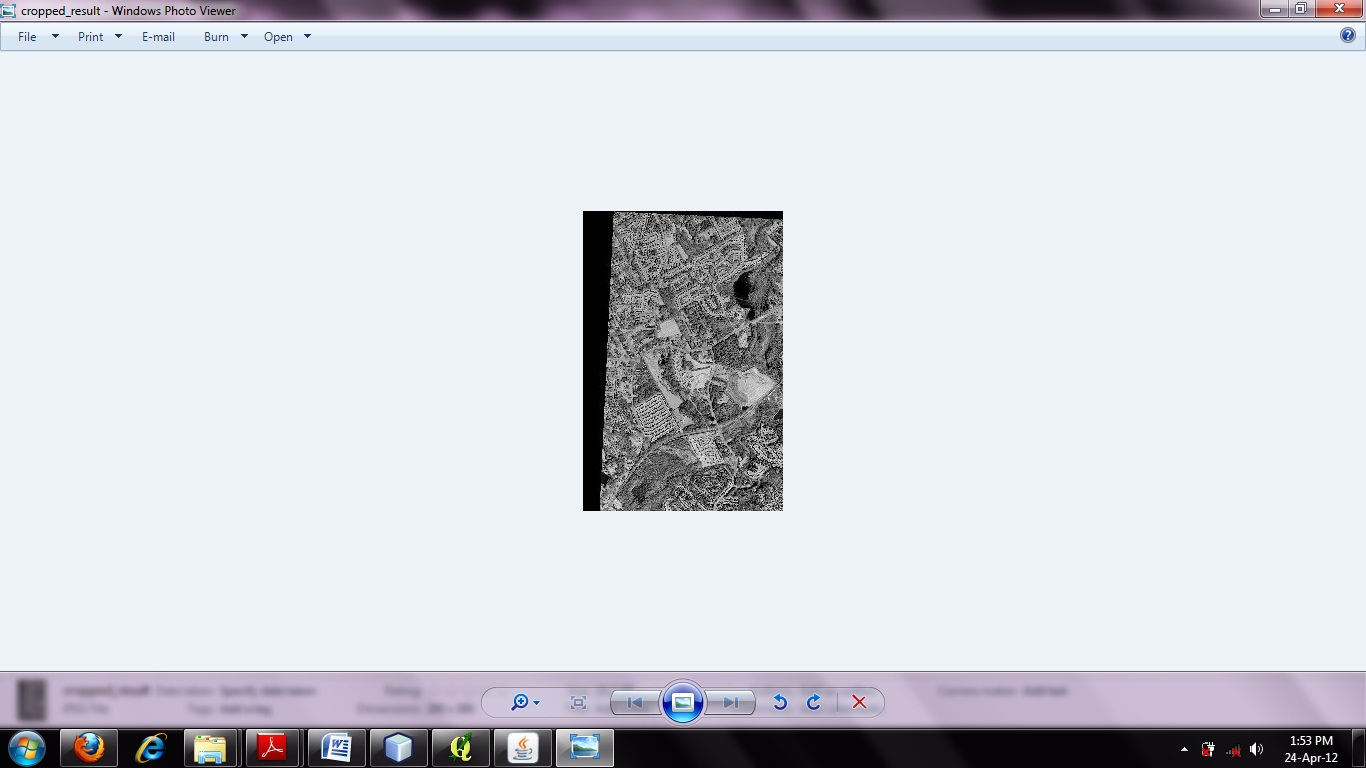
\includegraphics[scale=0.43] {15.jpg}
  \caption[Screenshot - Output Image]{Cropped Result}
\end{center}
\end{figure}
Description: Here is the output of  cropped TIFF file.That stores in Local directory of user.

\newpage
\begin{figure}[h]
\begin{center}
  % Requires \usepackage{graphicx}
  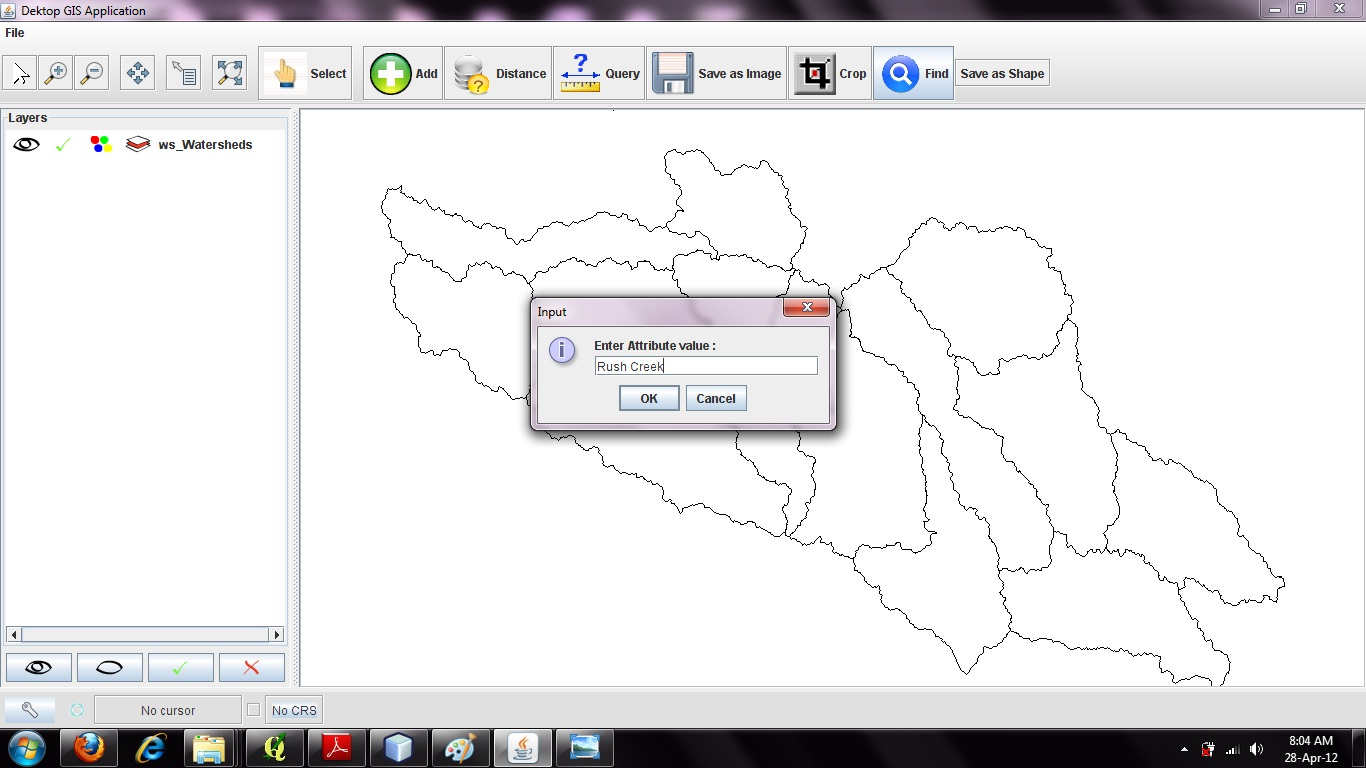
\includegraphics[scale=0.43] {16.jpg}
  \caption[Screenshot - Find]{Find the feature}
\end{center}
\end{figure}
Description: User can find the country/state from the opened Map using field name  stored in Attribute Table

\newpage
\begin{figure}[h]
\begin{center}
  % Requires \usepackage{graphicx}
  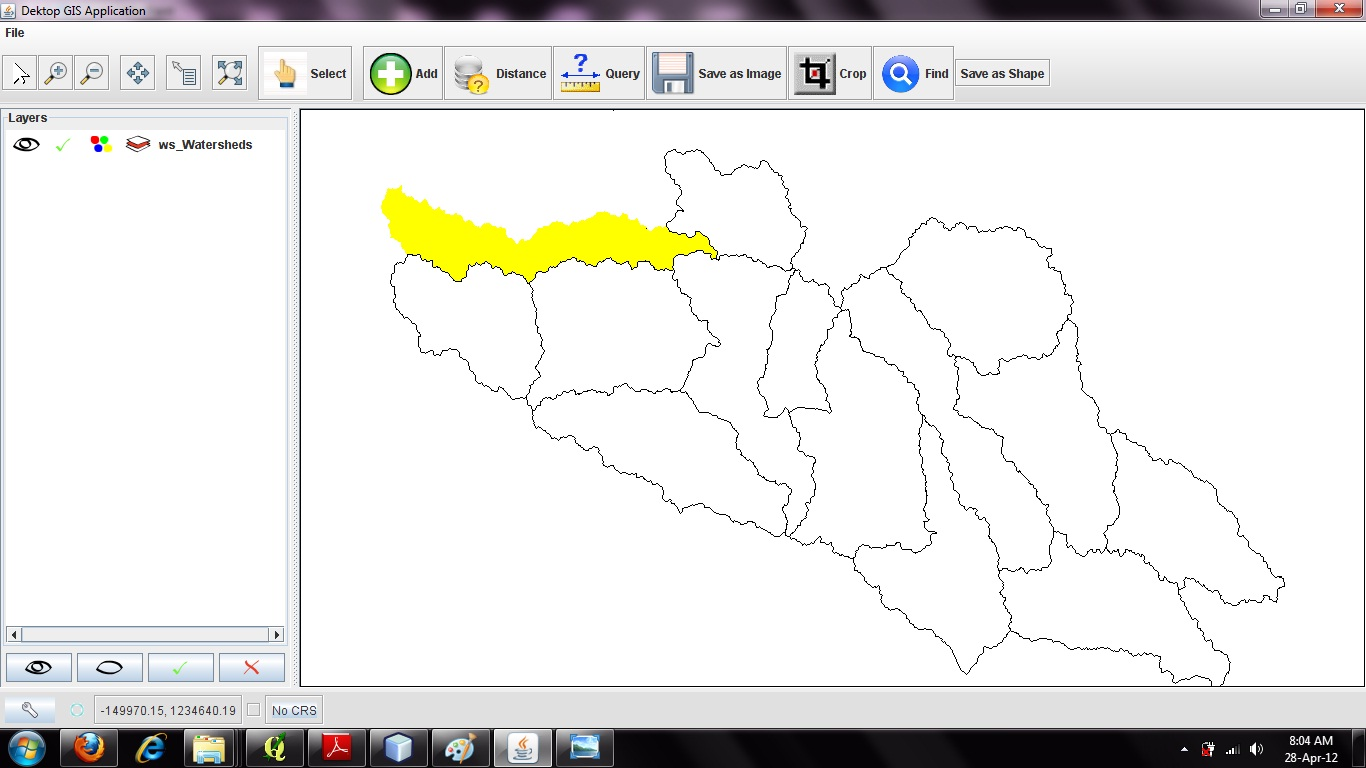
\includegraphics[scale=0.43] {17.jpg}
  \caption[Screenshot - Result of Finding]{Result of finding}
\end{center}
\end{figure}
Description: Here is the outcome of finding the feature name “Algeria”. The part is highlighted in Map.
\newpage

\begin{figure}[h]
\begin{center}
  % Requires \usepackage{graphicx}
  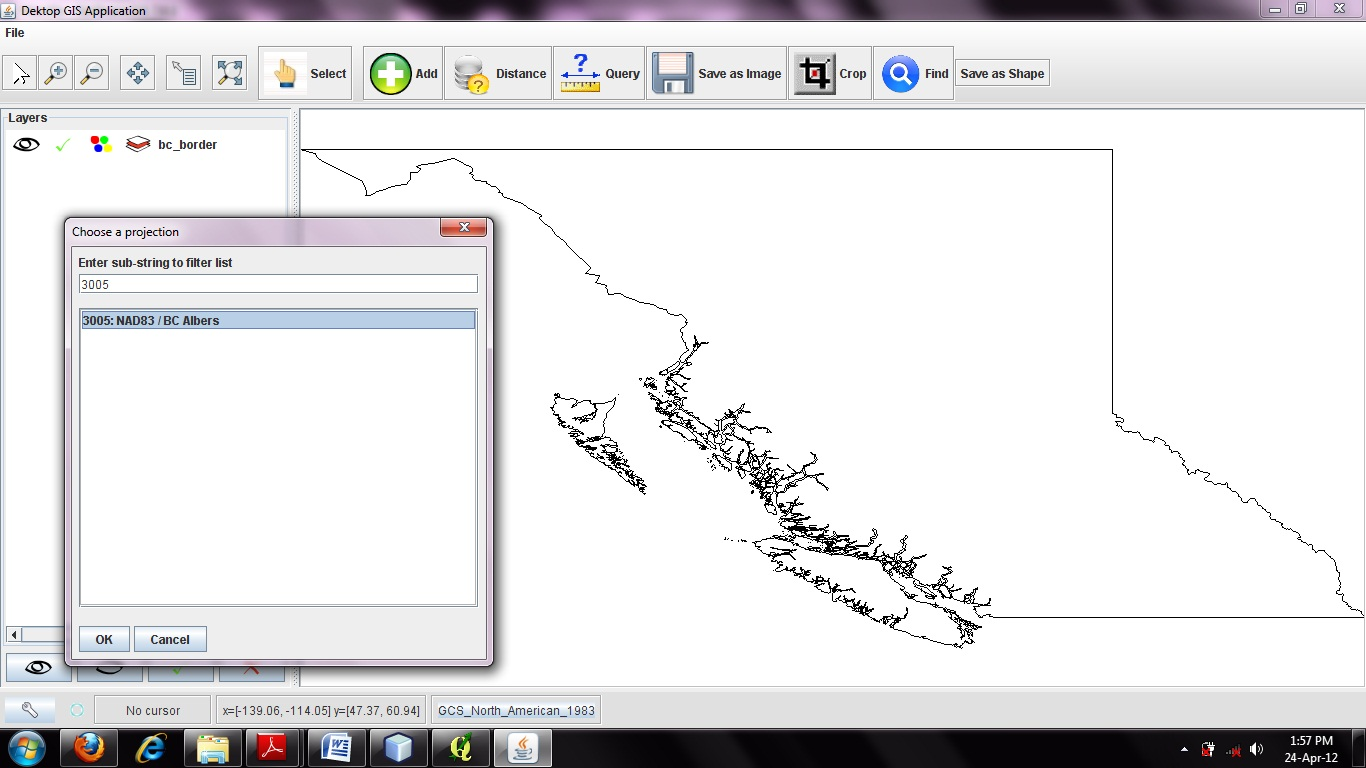
\includegraphics[scale=0.43] {18.jpg}
  \caption[Screenshot - Changing The CRS]{Changing the Coordinate Reference System}
\end{center}
\end{figure}
Description: Above user can change the CRS of shape file if its not proper so that the projection of the map can be properly displayed.
\newpage
\begin{figure}[h]
\begin{center}
  % Requires \usepackage{graphicx}
  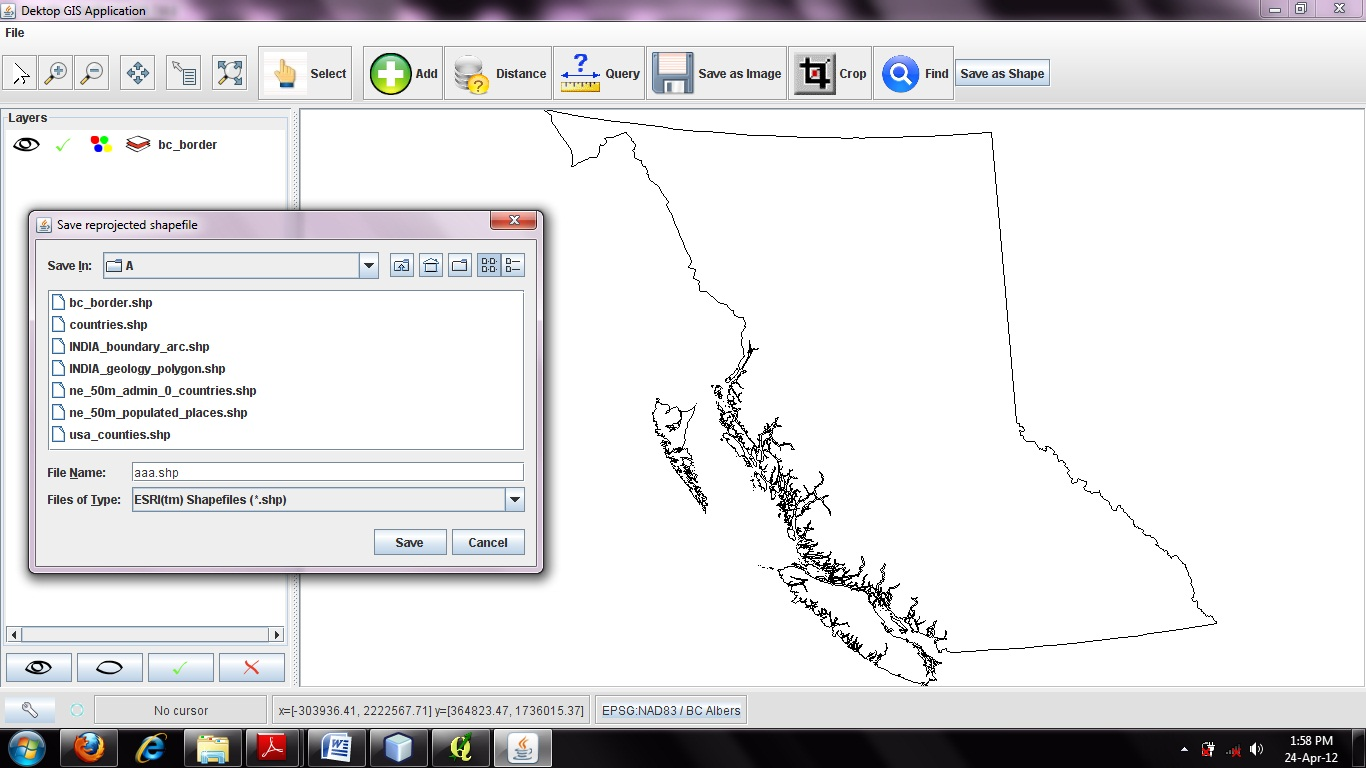
\includegraphics[scale=0.43] {19.jpg}
  \caption[Screenshot - Save as Shape]{Save as Shape file}
\end{center}
\end{figure}
Description: User can save the reprojected file as shape file in local directory and use it for future purpose.

\newpage
\begin{figure}[h]
\begin{center}
  % Requires \usepackage{graphicx}
  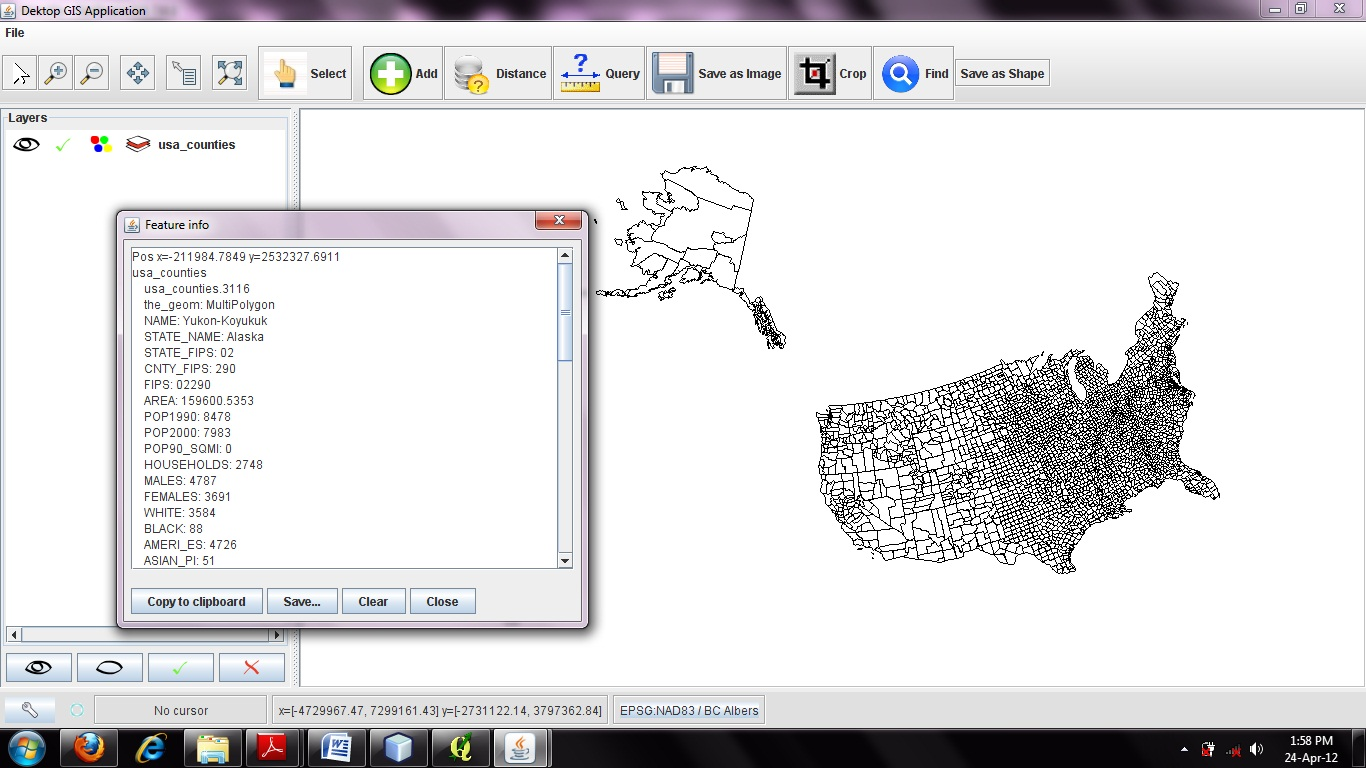
\includegraphics[scale=0.43] {20.jpg}
  \caption[Screenshot - Feature Info]{Features in selected Layers}
\end{center}
\end{figure}
Description: Above is outcome of the process when user click on some point in map using feature selection tool in Map.The all attributes entry related to that point is displayed in figure.
